\documentclass[msc,deptreport,cs]{infthesis} % Do not change except to add your degree (see above).

%% Imports poached from frankly
%% STILL can't find what makes \figrule work
\usepackage{natbib}
\usepackage{mathpartir}
\usepackage{amsmath}
\usepackage{amsfonts}
\usepackage{thmtools,thm-restate}
\usepackage{comment}
\usepackage{flushend}
\usepackage{listings}

%% \usepackage{beramono}

%% \lstdefinestyle{mystyle}{
%%     %% backgroundcolor=\color{backcolour},
%%     %% commentstyle=\color{codegreen},
%%     %% keywordstyle=\color{magenta},
%%     %% numberstyle=\tiny\color{codegray},
%%     %% stringstyle=\color{codepurple},
%%     breakatwhitespace=false,
%%     breaklines=true,
%%     captionpos=b,
%%     keepspaces=true,
%%     %% numbers=left,
%%     %% numbersep=5pt,
%%     showspaces=false,
%%     showstringspaces=false,
%%     showtabs=false,
%%     tabsize=2,
%%     %% basicstyle=\small\ttfamily
%%     basicstyle=\ttfamily\footnotesize,
%%     %% breaklines=true
%% }

%% \lstset{style=mystyle}

\lstset{
  basicstyle=\small\ttfamily,
  breaklines=true
}

\usepackage{stmaryrd}
\usepackage{natbib}
\usepackage{xspace}
%% \usepackage[pdftex,
%%             pdfauthor={Sam Lindley, Conor McBride, and Craig McLauglin},
%%             pdftitle={Doo bee doo bee doo}]{hyperref}
%\hypersetup{colorlinks=true,citecolor=blue,linkcolor=blue}
%% \hypersetup{colorlinks=true,allcolors=black}
\usepackage[usenames,dvipsnames]{xcolor}
\usepackage{url}

% get rid of hypertext link on \citeauthor
\usepackage{etoolbox}

\usepackage{amssymb}

\usepackage{mathtools} % allows flush-left align environments and paired
                       % delimiters.
                       %


% Theorem environments
\newtheorem{theorem}{Theorem}
\newtheorem{proposition}[theorem]{Proposition}
\newtheorem{definition}[theorem]{Definition}
\newtheorem{prop}[theorem]{Proposition}
\newtheorem{lemma}[theorem]{Lemma}
\newtheorem{corollary}[theorem]{Corollary}


%% abstract for inline code
\newcommand{\code}[1]{\lstinline{#1}}


%%%%%%%%%%%%%%%%%%%%%%%%%%%%%%%%%%%%%%%%%%%%%%%%%
%% Start of inference rules typesetting business
%%%%%%%%%%%%%%%%%%%%%%%%%%%%%%%%%%%%%%%%%%%%%%%%%

\DeclarePairedDelimiter{\ceil}{\lceil}{\rceil}

\newcommand{\todo}[1]
           {{\par\noindent\small\color{RoyalPurple}
  \framebox{\parbox{\dimexpr\linewidth-2\fboxsep-2\fboxrule}
    {\textbf{TODO:} #1}}}}

\newcommand{\interrupt}[1]{!(#1)}

\newcommand{\fighead}{\textbf}

\newcommand{\lameff}{$\lambda_{\text{eff}}$\xspace}
\newcommand{\lameffrow}{$\lambda_{\text{eff}}^\rho$\xspace}
\newcommand{\feff}{$F_\textrm{eff}$\xspace}
\newcommand{\impeff}{Implicit \lameff}
\newcommand\Frank{\emph{Frank}\xspace}

\newcommand\Cse{\textbf{Case}}

\newcommand{\set}[1]{\{#1\}}
\newcommand{\many}{\overline}
\newcommand{\opt}[1]{#1^?}
\newcommand{\medvert}{\mid}

\newcommand{\sem}[1]{\llbracket{#1}\rrbracket}
\newcommand{\seml}{\left\llbracket}
\newcommand{\semr}{\right\rrbracket}

\newcommand{\mdo}{~\textbf{do}~}
\newcommand{\seq}{~\textbf{;}~}
\newcommand{\assn}[2]{{#1}~\leftarrow~{#2}}
\newcommand{\func}[2]{\text{#1}~{#2}}

\newcommand{\deno}[1]{\sem{#1}\rho}
\newcommand{\denoex}[2]{\sem{#1}#2}
\newcommand{\pc}[1]{\llparenthesis{#1}\rrparenthesis}

\newcommand{\TyVar}{\mathit{Var}}
\newcommand{\dom}{\mathit{dom}}
%\newcommand{\sub}{\subseteq}
\newcommand{\Star}{{\Large$\star$}}

\newcommand{\reducesto}{\longrightarrow}

\newcommand\ba{\begin{array}}
\newcommand\ea{\end{array}}

\newcommand{\bl}{\ba[t]{@{}l@{}}}
\newcommand{\el}{\ea}

\newcommand{\bstack}{\begin{array}[t]{@{}l@{}}}
\newcommand{\estack}{\end{array}}

\newenvironment{equations}{\[\ba{@{}r@{~}c@{~}l@{}}}{\ea\]\ignorespacesafterend}
\newenvironment{eqs}{\ba{@{}r@{~}c@{~}l@{}}}{\ea}

\newenvironment{clauses}{\ba{@{}l@{~}c@{~}l@{}}}{\ea}

\newenvironment{syn}{\ba{@{}l@{~}r@{~}c@{~}l@{}}}{\ea}

\newenvironment{syntax}{\[\ba{@{}l@{~}r@{~}c@{~}l@{}}}{\ea\]\ignorespacesafterend}

\newcommand{\judgeword}[1]{~\mathbf{#1}~}

%\renewcommand{\sig}{\Sigma}
%\renewcommand{\sigs}{\Sigma s}
\newcommand{\sigentails}[1]{\mathbin{[{\text{\scriptsize ${#1}$}}]\hspace{-0.4ex}\text{-\!-}}\,}

%% \newcommand{\sigmodels}[1]{\mathbin{[{\text{\scriptsize ${#1}$}}]\!\mathord{=}}\,}
% \newcommand{\sigentails}[1]{\vdash_{#1}}

\newcommand{\val}[3]  {#1 \vdash {#2} : {#3}}

\newcommand{\rt}[1]{\langle{#1}\rangle}   % returner type

\newcommand{\valg}{\val{\Gamma}}

%% \newcommand{\is}[4]  {#1 \sigentails{#2} {#3} \judgeword{is} {#4}}
%% \newcommand{\isgs}{\is{\Gamma}{\sigs}}

%% \newcommand{\cdoes}[4]{#1 \sigentails{#2} {#3} \judgeword{has} {#4}
%% \newcommand{\cdoesgs}{\cdoes{\Gamma}{\sigs}}


%% some options for rendering bidirectional typing judgements

%% \newcommand{\inferbase}[4]{#2 \mathbin{#1} {#3} \in {#4}}
%% \newcommand{\checkbase}[4]{#2 \mathbin{#1} {#3} \ni {#4}}
%% \newcommand{\patbase}[4]{{#3} \mathbin{:} {#2} \mathbin{#1} {#4}}

\newcommand{\kindcheckbase}[3]{#2 \mathbin{#1} #3} % For well-kindedness of types
\newcommand{\inferbase}[5]{#1; #3 \mathbin{#2} {#4} \Rightarrow {#5}}
\newcommand{\checkbase}[5]{#1; #3 \mathbin{#2} #5 \mathbin{:} #4}
\newcommand{\patbase}[5]{{#1} \vdash {#4} \mathbin{:} {#3} \mathbin{#2} {#5}}
\newcommand{\bindbase}[4]{{#3} \mathbin{:} {#2} \mathbin{#1} {#4}}

%% \newcommand{\inferbase}[4]{#2 \mathbin{#1} {#3} \Rightarrow {#4}}
%% \newcommand{\checkbase}[4]{#2 \mathbin{#1} {#4} \Leftarrow {#3}}
%% \newcommand{\patbase}[4]{{#3} \mathbin{:} {#2} \mathbin{#1} {#4}}

%% \newcommand{\inferbase}[4]{#2 \mathbin{#1} {#3} \uparrow {#4}}
%% \newcommand{\checkbase}[4]{#2 \mathbin{#1} {#4} \downarrow {#3}}
%% \newcommand{\patbase}[4]{{#3} \mathbin{:} {#2} \mathbin{#1} {#4}}

%% \newcommand{\inferbase}[4]{#2 \mathbin{#1} {#3} \judgeword{infers} {#4}}
%% \newcommand{\checkbase}[4]{#2 \mathbin{#1} {#3} \judgeword{checks} {#4}}
%% \newcommand{\patbase}[4]{{#2} \judgeword{matches} {#3} \mathbin{#1} #4}

\newcommand{\makes}[5]{\inferbase{#1}{\sigentails{#3}}{#2}{#4}{#5}}
\newcommand{\has}[5]{\checkbase{#1}{\sigentails{#3}}{#2}{#4}{#5}}
\newcommand{\does}[4]{\checkbase{#1}{\vdash}{#2}{#3}{#4}}
\newcommand{\can}[4]{\makes{\kenv}{#1}{#2}{#3}{#4}}

\newcommand{\effs}[2]{{#1} \judgeword{does} {#2}}


% redefinitions for cbv type system
\newcommand{\kindchecks}[2]{\kindcheckbase{\vdash}{#1}{#2}} % Checks that a type is well-kinded
\newcommand{\infers}{\makes}
\newcommand{\checks}{\has}
\newcommand{\checksdef}{\does}
\newcommand{\matchesc}{\matches}
\newcommand{\matchesck}{\matchesc{\kenv}}

\newcommand{\infersk}{\makes{\kenv}}
\newcommand{\checksk}{\has{\kenv}}
\newcommand{\checksdefk}{\does{\kenv}}

\newcommand{\kindchecksk}{\kindchecks{\kenv}} % Checks that a type is well-kinded
\newcommand{\inferskgs}{\makes{\kenv}{\Gamma}{\sigs}}
\newcommand{\checkskgs}{\has{\kenv}{\Gamma}{\sigs}}
\newcommand{\checksdefkg}{\does{\kenv}{\Gamma}}


\newcommand{\adj}{\Delta}
\newcommand{\adapt}{\Theta}
\newcommand{\ext}{\Xi}
\newcommand{\sigs}{\Sigma}
\newcommand{\sig}{I}

\newcommand{\seed}{\sigma}

\newcommand{\effbox}[1]{[#1]}

\newcommand{\key}[1]{\mathbf{#1}} % keyword
\newcommand{\var}{\mathit}        % local variable or meta variable
\newcommand{\defaultvarname}[0]{x}

\newcommand{\op}{\mathsf}  % operator (command or computation)
\newcommand{\con}{\mathsf} % constructor (type or data)
\newcommand{\inter}{\mathsf} % interface
\newcommand{\str}[1]{\textrm{``#1''}} % string literal


\newcommand{\handleSymbol}{\rightarrow}
\newcommand{\handle}[2]{{#1} \handleSymbol {#2}}

\newcommand{\thunk}[1]{\{{#1}\}}

\newcommand{\force}[1]{{#1}!}

\newcommand{\emptylist}{[]}
\newcommand{\cons}{\mathbin{::}}
\newcommand{\concat}{\,\texttt{++}\,} %mathbin{+\!+}}
%\newcommand{\snoc}{\mathbin{:<}}
\newcommand{\snoc}{\ }


\newcommand{\NN}{\mathbb{N}}

\newcommand\slab[1]{(\textrm{#1})}

\newcommand{\ev}{E}
\newcommand{\evd}{\varepsilon}

\newcommand{\effin}[1]{\langle {#1} \rangle}
\newcommand{\effout}[1]{[{#1}]}

\newcommand{\nowt}{\emptyset}
\newcommand{\id}{\iota}
\newcommand{\pid}{\var{s}} % Pattern identity variable

\newcommand{\EC}{\mathcal{E}}
\newcommand{\EF}{\mathcal{F}}
\newcommand{\PC}{\mathcal{P}} % Syntactic phrase class for af operation
\newcommand{\venv}{\theta}

\newcommand{\freeze}{\ceil}

\newcommand{\uc}{\mathord{\downarrow}}
\newcommand{\cu}{\mathord{\uparrow}}

\newcommand{\redtou}{\leadsto_{\mathrm{u}}}
\newcommand{\redtoc}{\leadsto_{\mathrm{c}}}
\newcommand{\stepsto}{\longrightarrow}

\newcommand{\stepstou}{\longrightarrow_{\mathrm{u}}}
\newcommand{\stepstoc}{\longrightarrow_{\mathrm{c}}}

\newcommand{\sigat}{\mathbin{@}}

\newcommand{\meta}{\mathsf}
\newcommand{\level}{\meta{level}}
\newcommand{\af}{\meta{af}}
\newcommand{\handles}{~\meta{handles}~}

\newcommand{\poised}{~\meta{poisedfor}~}
\newcommand{\insts}{\meta{inst}}
\newcommand{\remap}{\meta{remap}}

\newcommand{\sigyields}[1]
           {\mathbin{\text{-\!-\!}[{\text{\scriptsize ${#1}$}}]\,}}

\newcommand{\matches}[5]{\patbase{#1}{\sigyields{#4}}{#2}{#3}{#5}}
\newcommand{\matchesv}[4]{\patbase{#1}{\dashv}{#2}{#3}{#4}}
\newcommand{\matchesvk}{\matchesv{\kenv}}

\newcommand{\bindsv}[4]{\bindbase{\dashv}{#2 \leftarrow #3}{#1}{#4}}
\newcommand{\bindsc}[5]{\bindbase{\sigyields{#4}}{#2 \leftarrow #3}{#1}{#5}}

\newcommand{\letin}[4][\defaultvarname]
           {\key{let}\;{#1}:{#2}={#3}\;\key{in}\;{#4}}
\newcommand{\letxin}[3][\defaultvarname]
           {\key{let}\;{#1}={#2}\;\key{in}\;{#3}}
\newcommand{\letrec}[4][f]{\key{letrec}~\many{{#1}:{#2} = {#3}}~\key{in}~{#4}}
\newcommand{\letrecU}[3][f]{\key{letrec}~\many{{#1} = {#2}}~\key{in}~{#3}}
\newcommand{\Gt}{\theta} % Substitution meta variable
\newcommand{\submap}[2]{{{#1}\vDash{#2}}}
\newcommand{\sub}[4]{#1 \vdash {{#2}:\submap{{#3}}{{#4}}}}
\newcommand{\subk}{\sub{\kenv}}
\newcommand{\subext}[2]{{{#1}{#2}}}
\newcommand{\subst}[3][\defaultvarname]{{#2}[{#3}/{#1}]}

% Frank letrec substitution
\newcommand{\recsub}[5][f]
      {[\many{\cu (\thunk{\many{\many{#2}\mapsto\letrec[{#1}]{#5}{#3}{#4}}}
            : {#5})/{#1}}]}


%%%% START inference rule system for action of adjustment on ability %%%%
\newcommand{\semi}{;}
\newcommand{\kenv}{\Phi}  % kind environment
\newcommand{\kenva}{\Psi} % another kind environment
%% \newcommand{\kenv}{\mathcal{T}} % kind environment
\newcommand{\ienv}{\Omega} % Instance environment
\newcommand{\adjact}[3]{{#1}\vdash{#2}\dashv{#3}}
\newcommand{\adpcom}[5]{{{#1}\vdash{#2}({#3} \to {#4})\dashv{#5}}}
\newcommand{\itrbnd}[5]{{{#1}\vdash{#2}:{#3}\dashv{#4}\semi{#5}}}
% \newcommand{\wf}[2]{{{#1}\vdash{#2}}}
\newcommand{\itrinst}[4]{{{#1}\vdash{#2}:{#3}\dashv{#4}}}

%%% END inference rule system for action of adjustment on ability %%%%%

% Untyped machine letrec substitution
\newcommand{\recsubst}[5]
 {{#1}[\many{(\thunk{\many{\many{#2} \mapsto \letrecU{#3}{#4}}}:{#5})/f}]}

%% Abstract machine commands
% Typing
\newcommand{\HAbs}[2]{{{#1}\to{#2}}}

\newcommand{\fail}{\textbf{fail}}

%% Translation function: Frank Terms to Untyped A-Normal Form
\newcommand{\UANF}[1]{{\llbracket{{#1}}\rrbracket}}

% Terms
\newcommand{\mtrns}[3][]{{#2} & \Rightarrow^{#1} & {#3}} % For array env
\newcommand{\mtrnsR}[3][]{{#2}\Rightarrow^{#1}{#3}}

\newcommand{\confg}[2]{{\langle{{#1}},{{#2}}\rangle}}
\newcommand{\term}[3]
           {{\langle{{#1}},{{#2}}\rangle\downarrow{#3}}}

\newcommand{\admin}[2]{{\langle{{#1}}\mid{{#2}}\rangle}}
\newcommand{\mat}[3]
           {{\langle{{#1}}\mid{{#2}}\mid{{#3}}\rangle}}
\newcommand{\matc}[5]
        {{\langle{{#1}}\mid{{#2}}\mid{{#3}}\mid{{#4}}\mid{{#5}}\rangle}}

\newcommand{\msub}[3][\defaultvarname]{{#2}[{#1}\mapsto{#3}]}

\newcommand{\FHan}[4][\many{\effin{\adj}}]{{({#2}:{#1},{#3}\mid{#4})}}
\newcommand{\FSeq}[2][\defaultvarname]
           {{({#1}.{#2})}}
\newcommand{\SCons}[2]{{{#1}\circ{#2}}}


\newcommand{\HSHan}[5][C]{{{#2}\circ({#3},{#1},{#4}\mid{#5})}}
\newcommand{\HSSeq}[4][\defaultvarname]
           {{#2}\circ({#1}:{#3}.{#4})}
\newcommand{\HSCons}[2]{{{#1}\circ{#2}}}
\newcommand{\NF}[2]{{{#1}~\star~{#2}}}

\newcommand{\evalto}{\Longrightarrow}


\newcommand{\para}[1]{\paragraph{#1.}}

\newcommand{\gor}{\mid}
\newcommand{\pipe}{\texttt{|}}


%%%%%%%%%%%%%%%%%%%%%%%%%%%%%%%%%%%%%%%%%%%%%%%%%
%% End of inference rules typesetting business
%%%%%%%%%%%%%%%%%%%%%%%%%%%%%%%%%%%%%%%%%%%%%%%%%






%%%%%%%%%%%%%%%%%%%%%%%%%%%%%%%%%%%%%%%%
%% Start of main text
%%%%%%%%%%%%%%%%%%%%%%%%%%%%%%%%%%%%%%%%

\begin{document}
\begin{preliminary}

\title{Asynchronous Effect Handling}

\author{Leo Poulson}

\abstract{
Abstract
}

\maketitle

\section*{Acknowledgements}
thanks!

\tableofcontents

\end{preliminary}

\chapter{Programming in Frank}

\section{Effects and Effect Handling}

\paragraph*{Interfaces and Operations}

Frank encapsulates effects through \emph{interfaces}, which offer
\emph{commands}. For instance, the \code{State} effect (interface) offers two
operations (commands), \code{get} and \code{put}. In Frank, this translates to

\begin{lstlisting}
  interface State X = get : X
                    | put : X -> Unit
\end{lstlisting}

The type signatures of the operations mean that \code{get} is a 0-ary operation
which is \emph{resumed} with a value of type \code{X}, and \code{put} takes a value of
type \code{X} and is resumed with \code{unit}. Programs get access to an interface's
command by including them in the \emph{ability} of the program. Commands are
invoked just as normal functions;

\begin{lstlisting}
  xplusplus : {[State Int] Unit}
  xplusplus! = let x = get! in put (x + 1)
\end{lstlisting}

\noindent This familiar program increments the integer in the state by 1.

\paragraph*{Handling Operations}

Traditioanl functions in Frank are a specialisation of Frank's handlers; that is
to say, functions are handlers that handle no effects. A handler for an
interface pattern matches \emph{on the operations} that are invoked, as well as
on the \emph{values} that the computation can return. Furthermore, the handler
gets access to the \emph{continuation} of the calling function as a first-class
value. Consider the handler for \code{State};

\begin{lstlisting}
  runState : {<State S> X -> S -> X}
  runState <get -> k>   s = runState (k s) s
  runState <put s -> k> _ = runState (k unit) s
  runState x            _ = x
\end{lstlisting}

\noindent The type of \code{runState} expresses that the first argument is a
computation that can perform \code{State S} effects and will eventually return a
value of type \code{X}, whilst the second argument is a value of type \code{S}.
%could remove this below line...
The \code{State S} effect is then \emph{removed} from the first argument.

What happens when we run \code{runState xplusplus! 0}?

%% Frank's realisation of effects is through \emph{interfaces} which offer
%% \emph{commands}. For instance, the \code{State} effect (interface) offers two
%% operations (commands), \code{get} and \code{put}. In Frank, this translates to

%% \begin{lstlisting}
%%   interface State X = get : X
%%                     | put : X -> Unit
%% \end{lstlisting}

%% The type signatures of the operations mean that \code{get!}, when handled, will
%% be a value of type \code{X}, whilst \code{put x} once handled will be a value of
%% type \code{Unit}.

%% \code{get} and \code{put} are given meaning by defining a \emph{handler} for the
%% \code{State} interface. Handlers in Frank are very simple things; they take as
%% argument a computation that can perform effects. The handlers then pattern match
%% \emph{on the operations} that are invoked, as well as on the \emph{values} that the
%% computation can return. What makes effects not just a special kind of value is
%% that they also offer the \emph{continuation} of the caller as a first-class
%% value.

%% Here we display the handler for \code{State};

%% \begin{lstlisting}
%%   runState : {<State X> Y -> X -> Y}
%%   runState <get -> k>   s = runState (k s) s
%%   runState <put s -> k> _ = runState (k unit) s
%%   runState y            _ = y
%% \end{lstlisting}


\section{Concurrency}
\label{sec:concurrency}

Frank is a single-threaded language. It is fortunate, then, that effect handlers
give us a malleable way to run multiple program-threads ``simultaneously'' \todo
{This is poorly written --- fix}.

This is because the invocation of an operation not only offers up the
operation's payload, but also the \emph{continuation} of the calling
computation. The handler for this operation is then free to do what it pleases
with the continuation. For many effects, such as \code{getState}, nothing
interesting happens to the continuation; in the case of \code{getState}, it is
resumed with the value in state. But these continuations are first-class; they
can resumed, sure, but also stored elsewhere or even thrown away. As such, by
handling \code{Yield} operations, we easily pause and switch between several
threads.

\subsection{Simple Scheduling}

We introduce some simple program threads and some scheduling multihandlers, to
demonstrate how subtly different handlers generate different scheduling
strategies.

\begin{lstlisting}
interface Yield = yield : Unit

words : {[Console, Yield] Unit}
words! = print "one "; yield!; print "two "; yield!; print "three "; yield!

numbers : {[Console, Yield] Unit}
numbers! = print "1 "; yield!; print "2 "; yield!; print "3 "; yield!
\end{lstlisting}

First note the simplicity of the \code{Yield} interface; we have one operation
supported, which looks very boring; the operation \code{yield!} will just return
unit --- of course, it is the way we \emph{handle} yield that is more
interesting.

\begin{lstlisting}
-- Runs all of the LHS first, then the RHS.
scheduleA : {<Yield> Unit -> <Yield> Unit -> Unit}
scheduleA <yield -> m> <n> = scheduleA (m unit) n!
scheduleA <m> <yield -> n> = scheduleA m! (n unit)
scheduleA _ _ = unit

-- Lets two yields synchronise, then handles both
scheduleB : {<Yield> Unit -> <Yield> Unit -> Unit}
scheduleB <yield -> m> <yield -> n> = scheduleB (m unit) (n unit)
scheduleB <yield -> m> <n> = scheduleB (m unit) n!
scheduleB <m> <yield -> n> = scheduleB m! (n unit)
scheduleB _ _ = unit
\end{lstlisting}

\todo{Can maybe delete the 2nd and 3rd matches of scheduleB to make the point
  more clear?}

We see two multihandlers above. Each take two \code{yield}ing threads and
schedule them, letting one run at a time. \code{scheduleA} runs the first thread
to completion, and only then runs the second one; the first time that the second
thread \code{yield}s it is \emph{blocked}, and can no longer execute. As such,
the output of \code{scheduleA words! numbers!} is \code{one 1 two three 2 3
  unit}.

\code{scheduleB} is fairer and more profound. We run \code{scheduleB words!
  number!} and receive \code{one 1 two 2 three 3 unit}; \code{scheduleB} is fair
and will ``match'' the yields together. We step through slowly. First
\code{words!} will print \code{one}, then it will \code{yield}. At this point
--- recalling that multihandlers pattern match left-to-right --- the second
thread, \code{numbers!}, is allowed to execute. In the meantime, \code{words!}
is stuck as \code{<yield -> m>}; it cannot evaluate any further, it is
\emph{blocked}. Whilst \code{words} is blocked \code{numbers!} prints \code{1}
and then \code{yield}s. Great; now the first case matches. Both threads are
resumed and the process repeats itself.

\todo{ The second paragraph here is a more compelling explanation; maybe we can
  just get rid of all of the scheduleA business and /just/ have the scheduleB
  stuff? scheduleA is quite obvious i think whilst B is more subtle and compelling. }

\todo{ It's not true that it matches L-R as much as runs all computations L - R
  until they are all a command / value - fix this }

\subsection{Forking New Processes}

We can make use of Frank's higher-order effects to dynamically create new
threads at runtime. We strengthen the \code{Yield} interface by adding a new
operation \code{fork};

\begin{lstlisting}
  interface Co = fork : {[Co] Unit} -> Unit
               | yield : Unit
               | exit : Unit
\end{lstlisting}

The type of \code{fork} expresses that \code{fork} takes a suspended computation
that can perform further \code{Co} effects, and returns unit when handled. We
can now run programs that allocate new threads at runtime, such as the below

\begin{lstlisting}
forker : {[Console, Co [Console]] Unit}
forker! = print "Starting! ";
          fork {print "one "; yield!; print "two "};
          fork {print "1 "; yield!; print "2 "};
          exit!
\end{lstlisting}

We can now choose a strategy for handling \code{fork} operations; we can either
lazily run them, by finishing executing the current thread, or eagerly run them,
suspending the currently executing thread and running the forked process. The
handler for the former, breadth-first style of scheduling, is

\begin{lstlisting}
scheduleBF : {<Co> Unit -> [Queue Proc] Unit}
scheduleBF <fork p -> k> =
    enqueue (proc {scheduleBF (<Queue> p!)});
    scheduleBF (k unit)
scheduleBF <yield -> k> =
    enqueue (proc {scheduleBF (k unit)});
    runNext!
scheduleBF <exit -> _> =
    runNext!
scheduleBF unit =
    runNext!
\end{lstlisting}

Notice the use of the \code{Queue} effect; we have to handle the computation
\code{scheduleBF forker!} with a handler for \code{Queue} effects afterwards.
Moreover, notice how concisely we can express the scheduler; this is due to the
handler having access to te continuation of the caller, and treating it as a
first-class object that can be stored elsewhere. We can see a diagram of how
\code{scheduleBF} treats continuations in Figure \ref{fig:scheduleBF}, and a
similar diagram of how the depth-first handling differs in Figure \ref{fig:scheduleDF}.

\begin{figure}[t]
  \centering
  \begin{subfigure}
    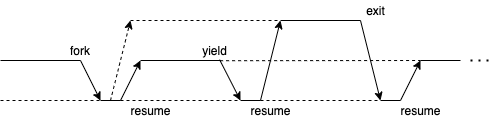
\includegraphics[width=0.8\textwidth]{imgs/scheduleBF.png}
    \caption{Breadth-First scheduling}
    \label{fig:scheduleBF}
  \end{subfigure}
  \begin{subfigure}
    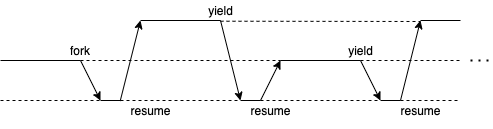
\includegraphics[width=0.8\textwidth]{imgs/scheduleDF.png}
    \caption{Depth-First scheduling}
    \label{fig:scheduleDF}
  \end{subfigure}
\end{figure}

\chapter{Formalisation of Frank}


\begin{figure}  %\figrule
\[
\ba{@{}c@{}}
\ba{@{}c@{\quad\quad}c@{}}
\begin{syn}
  \slab{data types}            & D \\
  \slab{value type variables}  & X \\
  \slab{effect type variables} & E \\
  \slab{value types}           & A, B   &::= & D~\overline{R} \\
                               &        &\gor& \thunk{C} \gor X \\
  \slab{computation types}     & C      &::= & \many{T \to}~G \\
  \slab{argument types}        & T      &::= & \effin{\adj}A \\
  \slab{return types}          & G      &::= & \effout{\sigs}A \\

  \slab{type binders}          & Z      &::= & X \gor [E]\\
  \slab{type arguments}        & R      &::= & A \gor [\Sigma]\\
  \slab{polytypes}             & P      &::= & \forall \overline{Z}.A \\
\end{syn}
&
\begin{syn}
  \slab{interfaces}           & I \\
  \slab{term variables}       & x, y, z, f \\
  \slab{instance variables}   & \pid, a, b, c \\
  \slab{seeds}                & \seed  &::= & \nowt \gor \ev \\
  \slab{abilities}            & \sigs  &::= & \seed\pipe\ext \\
  \slab{extensions}           & \ext   &::= & \id \gor \ext, \sig~\many{R} \\
  \slab{adaptors}             & \adapt &::= & \id \gor \adapt, \sig(S \to S') \\
  \slab{adjustments}          & \adj   &::= & \adapt\pipe\ext \\
  \slab{instance patterns}    & S      &::= & \pid \gor S \snoc a \\
  \slab{kind environments}    & \kenv,
                                \kenva &::= & \cdot \gor \kenv, Z \\
  \slab{type environments}    & \Gamma &::= & \cdot \gor \Gamma, x:A %\\
%                              &        &    & \hphantom{\cdot}
                                              \gor \Gamma, f:P\\
 \slab{instance environments} & \ienv  &::= & \pid:\sigs \gor \ienv, a:\sig~\many{R}\\
\end{syn} \\
\ea \\
\ea
\]
\\[0.25cm]

\caption{Types}
\label{fig:types}
%\figrule
\end{figure}




\begin{figure} %\figrule
\begin{syntax}
  %% \slab{monomorphic term variables} & x, y, z \\
  %% \slab{polymorphic term variables} & f \\
  \slab{constructors}               & k \\
  \slab{commands}                   & c \\
  \slab{uses}                 & m      &::= &
     x \gor f~\many{R} \gor m~\many{n} \gor \cu(n:A) \\
  \slab{constructions}        & n      &::= &
    \uc m \gor k~\many{n} \gor c~\many{R}~\many{n} \gor \thunk{e} \\
                              &        &\gor& \key{let}~f : P = n~\key{in}~n'
                                   \gor
                                   \key{letrec}~\many{f : P = e}~\key{in}~n \\
                              &        &\gor&  \effin{\adapt}~n \\
  \slab{computations}         & e      &::=& \many{\many{r} \mapsto n}
  \\
  \slab{computation patterns} & r      &::=& p
                                        \gor \effin{\handle{c~\many{p}\,}{z}}
                                        \gor \effin{x} \\
  \slab{value patterns}       & p      &::=& k~\many{p} \gor x        \\
\end{syntax}
\\[0.25cm]
%\textit{with} term variables $x$, $y$, $z$, polymorphic term variables $f$, constructors $k$, commands $c$\\[0.25cm]
\caption{Terms}
\label{fig:terms}
% \figrule
\end{figure}



\begin{figure} % \figrule
\flushleft
%% $\boxed{\kindchecksk{R}}$
%% \begin{mathpar}
%% \inferrule[K-Val]
%%   {\TyVar(A) \subseteq \kenv}
%%   {\kindchecksk{A}}

%% \inferrule[K-Eff]
%%   {\TyVar(\sigs) \subseteq \kenv}
%%   {\kindchecksk{[\sigs]}}
%% %
%% \end{mathpar}

$\boxed{\infersk{\Gamma}{\sigs}{m}{A}}$
\begin{mathpar}
\inferrule[T-Var]
  {
   x:A \in \Gamma}
  {\inferskgs{x}{A}}

\inferrule[T-PolyVar]
  {% \kindchecks{\kenv, \many{Z}}{A}\\
   \kindchecksk{\many{R}} \\
   f:\forall \many{Z}.A \in \Gamma}
  {\inferskgs{f~\many{R}}{A[\many{R}/\many{Z}]}}
\\
\inferrule[T-App]
  {\sigs' = \sigs \\
   (\adjact{\sigs}{\adj_i}{\sigs'_i})_i \\\\
   \inferskgs{m}{\thunk{\many{\effin{\adj}A \to}~ \effout{\sigs'}B}} \\
   (\checksk{\Gamma}{\sigs'_i}{A_i}{n_i})_i}
  {\infersk{\Gamma}{\sigs}{m~\many{n}}{B}}

\inferrule[T-Ascribe]
  {\checkskgs{A}{n}}
  {\inferskgs{\cu (n : A)}{A}}
%
\end{mathpar}

$\boxed{\checksk{\Gamma}{\sigs}{A}{n}}$
\begin{mathpar}
\inferrule[T-Switch]
  {\inferskgs{m}{A} \\ A = B}
  {\checkskgs{B}{\uc m}}

\inferrule[T-Data]
  {%(\kindchecksk{R_i})_i\\
   k~\many{A} \in D~\many{R} \\
   (\checkskgs{A_j}{n_j})_j}
  {\checkskgs{D~\many{R}}{k~\many{n}}}

\inferrule[T-Command]
  {\kindchecksk{\many{R}} \\
   c : \forall \many{Z}.\many{A \to}~ B \in \sigs \\
   (\checkskgs{A_j[\many{R}/\many{Z}]}{n_j})_j}
  {\checkskgs{B[\many{R}/\many{Z}]}{c~\many{R}~\many{n}}}

\inferrule[T-Thunk]
  {\checksdefkg{C}{e}}
  {\checkskgs{\thunk{C}}{\thunk{e}}}

\inferrule[T-Let]
  {P = \forall \many{Z}.A \\\\
   \checkbase{\kenv, \many{Z}}{\sigentails{\emptyset}}{\Gamma}{A}{n} \\
   \checksk{\Gamma, f : P}{\sigs}{B}{n'}}
  {\checkskgs{B}{\key{let}~f : P = n~\key{in}~n'}}

\inferrule[T-LetRec]
  {(P_i = \forall \many{Z}_i.\thunk{C_i})_i \\\\
   (\checkbase{\kenv, \many{Z}_i}{\vdash}{\Gamma, \many{f : P}}{C}{e_i})_i\\
   \checksk{\Gamma, \many{f : P}}{\sigs}{B}{n}}
  {\checkskgs{B}{\key{letrec}~\many{f : P = e}~\key{in}~n}}

\inferrule[T-Adapt]
  {\adjact{\sigs}{\adapt}{\sigs'} \\ \checksk{\Gamma}{\sigs'}{A}{n}}
  {\checkskgs{A}{\effin{\adapt}~n}}
\end{mathpar}

$\boxed{\checksdefkg{C}{e}}$
\begin{mathpar}
\inferrule[T-Comp]
  {(\matchesck{T_j}{r_{i,j}}{\sigs}{\exists \kenva_{i,j}.\Gamma'_{i,j}})_{i,j} \\
   (\checks{\kenv, (\kenva_{i,j})_j}{\Gamma, (\Gamma'_{i,j})_j}{\sigs}{B}{n_i})_i \\
   ((r_{i,j})_{i} \text{ covers } T_j)_j}
  {\checksdefkg{(T_j \to)_j~\effout{\sigs}B}{((r_{i,j})_j \mapsto n_i)_i}}
\end{mathpar}
\caption{Term Typing Rules}
\label{fig:term-typing}
% \figrule
\end{figure}



\begin{figure}[t]
%% \figrule
\begin{syntax}
\slab{uses}                    & m   &::= & \dots \mid \freeze{\EC[c~\many{R}~\many{w}]} \\
\slab{constructions}           & n   &::= & \dots \mid \freeze{\EC[c~\many{R}~\many{w}]} \\
\slab{use values}              & u   &::= & x \gor f~\many{R} \gor \cu (v : A) \\
\slab{non-use values}          & v   &::= & k~\many{w} \gor \thunk{e} \\
\slab{construction values}     & w   &::= & \uc u \gor v \\
\slab{normal forms}            & t   &::= & w \gor \freeze{\EC[c~\many{R}~\many{w}]} \\
\slab{evaluation frames}       & \EF &::= & [~]~\many{n}
                                      \gor  u~(\many{t},[~],\many{n})
                                      \gor  \cu([~]:A) \\
                               &     &\gor& \uc [~]
                                      \gor  k~(\many{w},[~],\many{n})
                                      \gor  c~\many{R}~(\many{w},[~],\many{n}) \\
                               &     &\gor& \key{let}~f: P = [~]~\key{in}~n
                                      \gor \effin{\adapt}~[~] \\
\slab{evaluation contexts}     & \EC &::= & [~] \gor \EF[\EC] \\
\end{syntax}
\caption{Runtime Syntax}
\label{fig:runtime-syntax}
%% \figrule
\end{figure}



\begin{figure}[t]
%% \figrule
\flushleft
$\boxed{\inferskgs{m}{A}}$ \quad $\boxed{\checkskgs{A}{n}}$
\begin{mathpar}
\inferrule[T-Freeze-Use]
  {\neg(\EC \handles c) \\
   \inferskgs{\EC[c~\many{R}~\many{w}]}{A}}
  {\inferskgs{\freeze{\EC[c~\many{R}~\many{w}]}}{A}}

\inferrule[T-Freeze-Cons]
  {\neg(\EC \handles c) \\
   \checkskgs{A}{\EC[c~\many{R}~\many{w}]}}
  {\checkskgs{A}{\freeze{\EC[c~\many{R}~\many{w}]}}}
\end{mathpar}
\caption{Frozen Commands}
\label{fig:frozen-typing}
%% \figrule
\end{figure}


\begin{figure}
%% \figrule
\flushleft
$\boxed{m \redtou m'} \quad \boxed{n \redtoc n'} \quad \boxed{m
    \stepstou m'} \quad \boxed{n \stepstoc n'}$
\begin{mathpar}
\inferrule[R-Handle]
  {% The type system should enforce this!
   %(\handles{\adj_j}{t_j})_j \\
   k = \min_i\,\{i \mid \exists \many{\venv}.(\bindsc{r_{i,j}}{\effin{\adj_j} A_j}{t_j}{\sigs}{\venv_j})_{j}\} \\
   (\bindsc{r_{k,j}}{\effin{\adj_j} A_j}{t_j}{\sigs}{\venv_j})_{j}}
   %% \forall i < k.\exists j.r_{i, j} \# t_j}
   %% l \text{~is minimal}}
  {\cu (\thunk{((r_{i,j})_j \to n_i)_i} : \thunk{\many{\effin{\adj} A \to}~\effout{\sigs}B})~\many{t} \redtou \cu ((\many{\venv}(n_k) : B)}

\inferrule[R-Ascribe-Use]
  { }
  {\cu(\uc u:A) \redtou u}

\inferrule[R-Ascribe-Cons]
  { }
  {\uc \cu (w : A) \redtoc w}

\inferrule[R-Let]
  { }
  {\key{let}~f:P = w~\key{in}~n \redtoc n[\cu (w : P)/f]}

\inferrule[R-LetRec]
  {\many{e = \many{\many{r} \to n}}}
  {%\vphantom{\many{\many{\many{\many{f}}}}}
   \key{letrec}~\many{f:P = e}~\key{in}~n' \redtoc
    n'[\many{\cu (\thunk{\many{\many{r} \to \key{letrec}~\many{f:P = e}~\key{in}~n}}: P)/f}]}

\inferrule[R-Adapt]
  { }
  {\effin{\adapt}~w \redtoc w}

\inferrule[R-Freeze-Comm]
  { }
  {c~\many{R}~\many{w} \redtoc \freeze{c~\many{R}~\many{w}}}\\

\inferrule[R-Freeze-Frame-Use]
  {\neg(\EF[\EC] \handles c)}
  {\EF[\freeze{\EC[c~\many{R}~\many{w}]}] \redtou \freeze{\EF[\EC[c~\many{R}~\many{w}]]}}

\inferrule[R-Freeze-Frame-Cons]
  {\neg(\EF[\EC] \handles c)}
  {\EF[\freeze{\EC[c~\many{R}~\many{w}]}] \redtoc \freeze{\EF[\EC[c~\many{R}~\many{w}]]}}

\\
\inferrule[R-Lift-UU]
  {m \redtou m'}
  {\EC[m] \stepstou \EC[m']}

\inferrule[R-Lift-UC]
  {m \redtou m'}
  {\EC[m] \stepstoc \EC[m']}

\inferrule[R-Lift-CU]
  {n \redtoc n'}
  {\EC[n] \stepstou \EC[n']}

\inferrule[R-Lift-CC]
  {n \redtoc n'}
  {\EC[n] \stepstoc \EC[n']}
\end{mathpar}

\caption{Operational Semantics}
\label{fig:small-step}
%% \figrule
\end{figure}


\begin{figure}[t]
%% \figrule
\flushleft
%\textit{Comp. pattern $r$ for $\langle \Delta \rangle A$ matches $u$ under
%amb. $\venv$ and binds $\venv$.}
$\boxed{\bindsc{r}{T}{t}{\sigs}{\venv}}$
\begin{mathpar}

\inferrule[B-Value]
  {\adjact{\sigs}{\adj}{\sigs'} \\\\ \bindsv{p}{A}{w}{\venv}}
  {\bindsc{p}{\effin{\adj}A}{w}{\sigs}{\venv}}

  \inferrule[B-Request]
    {%I~\many{R} \in \ext \\ %\capturesI{\Delta}{I}{\iota}\\
    \adjact{\sigs}{\adj}{\sigs'} \\
    \EC \poised c \\\\
    \adj = \adapt\pipe\ext \\
    c : \forall \many{Z}. \many{B \to}~B' \in \ext \\
    (\bindsv{p_i}{B_i}{w_i}{\venv_i})_i}
    {\bindsc{\effin{c~\many{p} \to z}}{\effin{\adj}A}
    {\freeze{\EC[c~\many{R}~\many{w}]}}{\sigs}{\many{\venv}[\cu (\thunk{x \mapsto \EC[x]} : \thunk{B' \to \effout{\sigs'}A})/z]}}

\inferrule[B-CatchAll-Value]
  {\adjact{\sigs}{\adj}{\sigs'}}
  {\bindsc{\effin{x}}{\effin{\adj}A}{w}{\sigs}{[\cu (\thunk{w}\mathord{:}\thunk{\effout{\sigs'}A})/x]}}
\\
\inferrule[B-CatchAll-Request]
  {
  \adjact{\sigs}{\adj}{\sigs'} \\
  \EC \poised c \\\\
  \adj = \adapt\pipe\ext \\
  c : \forall \many{Z}. \many{B \to}~B' \in \ext
  }
  {\bindsc{\effin{x}}{\effin{\adj}A}
  {\freeze{\EC[c~\many{R}~\many{w}]}}
  {\sigs}
  {[\cu (\thunk{\freeze{\EC[c~\many{R}~\many{w}]}}\mathord{:}\thunk{\effout{\sigs'}A})/x]}}

\end{mathpar}


%~~ \textit{Value pattern $p$ for type $A$ matches $w$ and binds $\venv$.}
%
$\boxed{\bindsv{p}{A}{w}{\venv}}$
\begin{mathpar}

\inferrule[B-Var]
  { }
  {\bindsv{x}{A}{w}{[\cu (w : A)/x]}}

\inferrule[B-Data]
  {k~\many{A} \in D~\many{R} \\
   (\bindsv{p_i}{A_i}{w_i}{\venv_i})_i}
 {\bindsv{k~\many{p}}{D~\many{R}}{k~\many{w}}{\many{\venv}}}
\end{mathpar}

\caption{Pattern Binding}
\label{fig:pattern-binding}
%% \figrule
\end{figure}



\chapter{Arbitrary Thread Interruption}

\section{Motivation}
\label{sec:interrupt-motivation}

One important part of our asynchronous effect handling system is the ability to
interrupt arbitrary computations.
%
This is essential for pre-emptive concurrency, which relies on being able to
suspend a computation \emph{without} the computation yielding.

%% Consider the following program;

%% \begin{lstlisting}
%% interface Stop = stop : Unit

%% interface Go = go : Unit

%% suspend : {<Stop, Go>Unit -> Unit -> Maybe {Unit} -> Unit}
%% suspend <stop -> k> <cont> _ =
%%     suspend (k unit) unit (just cont)
%% suspend <go -> k>   _      (just c)   =
%%     suspend (k unit) c! nothing

%% \end{lstlisting}

%% \noindent Here the first argument to \lstinline{suspend} performs
%% \lstinline{stop} and \lstinline{go} operations, which control the execution of
%% the second thread.

For instance, consider the two programs below;

\begin{lstlisting}
  controller : {[Stop, Go, Console] Unit}
  controller! = go!; stop!; print ``stop '';
                go!; stop!; print ``stop '';
                go!; stop!; print ``stop ''

  runner : {[Console] Unit}
  runner! = print ``1 ``; print ``2 ``; print ``3 '';
\end{lstlisting}

\noindent We ideally want a multihandler that can run these two programs in
parallel, such that the result will be \code{1 stop 2 stop 3 stop};
that is to say, the \code{stop} and \code{go} operations from \code{controller}
can control the execution of \code{runner}.

\section{Interruption with Yields}

One way we can get this behaviour is using the \code{Yield} interface. This
offers a single operation, \code{yield : Unit}. With this, we can write a
multihandler \code{suspend};

\begin{lstlisting}
runner : {[Console, Yield] Unit}
runner! = print "1 "; yield!; print "2 "; yield!; print "3 "; yield!

suspend : {<Yield> Unit -> <Stop, Go> Unit -> Maybe {[Console, Yield] Unit} -> [Console] Unit}
suspend <yield -> k> <stop -> l> _ = suspend unit (l unit) (just {k unit})
suspend <k>          <go -> l> (just res) = suspend (res!) (l unit) nothing
suspend <yield -> k> <m> maybe = suspend (k unit) m! maybe
suspend unit _ _ = unit
suspend _ unit _ = unit
\end{lstlisting}

\todo{Maybe make more concise?}
\todo{change to not be letter l cos it looks like a 1}

\noindent Running \code{suspend runner! controller! nothing} then prints out
\code{1 stop 1 2 stop 2 3 stop 3} as desired. So far so good; this works as
planned. However, observe that we had to change the code of the original runner
program to \code{yield} every time it prints. We would rather not have this
requirement; the threads should be suspendable without knowing in advance they
will be suspended, and thus without needing to explicitly \code{yield}.
Furthermore, see that the \code{yield} operation adds no more information; it is
just used as a placeholder operation; any operation would work. As such, we keep
searching for a better solution.

\section{Relaxing Catches}\label{sec:relaxingcatches}

The key to this lies in the catchall pattern, $\effin{x}$, and the pattern
binding rules of Figure \ref{fig:pattern-binding}.

Recall that the catchall pattern $\effin{x}$ matches either a value --- e.g.
\code{unit} --- or a command that is handled in the surrounding ability. For
instance, the pattern \code{<k>} in the code above matches either \code{unit}
or \code{<yield -> k>}. The variable \code{k} is then bound to
whatever this match is, leaving the (potentially) invoked effect unhandled. This
is expressed in the \textsc{B-CatchAll-Request} rule in Figure~\ref{fig:pattern-binding}.

Important to note is that only effects that are handled in that position are
able to be caught. \code{runner} also makes use of the \code{print} effect, but
these are not able to be caught by the catchall command. Formally, this is due
to the fourth requirement of \textsc{B-CatchAll-Request}; that the command $c$
that is invoked is a member of $\ext$.

\begin{figure}[t]
%% \figrule
%% \flushleft
%% \centering
%\textit{Comp. pattern $r$ for $\langle \Delta \rangle A$ matches $u$ under
%amb. $\venv$ and binds $\venv$.}
\begin{mathpar}

\inferrule[B-CatchAll-Request-Loose]
  {
  \adjact{\sigs}{\adj}{\sigs'} \\
  %% \EC \poised c \\\\
  %% \adj = \adapt\pipe\ext \\
  %% c : \forall \many{Z}. \many{B \to}~B' \in \ext
  }
  {\bindsc{\effin{x}}{\effin{\adj}A}
  {\freeze{\EC[c~\many{R}~\many{w}]}}
  {\sigs}
  {[\cu (\thunk{\freeze{\EC[c~\many{R}~\many{w}]}}\mathord{:}\thunk{\effout{\sigs'}A})/x]}}

\end{mathpar}

\caption{Updated \textsc{B-CatchAll-Request}}
\label{fig:loose-catchall-request}
%% \figrule
\end{figure}

As such, we propose to remove this constraint from \textsc{B-CatchAll-Request}.
The resulting rule can then be seen in Figure~\ref{fig:loose-catchall-request}.
This lets us update the previous \code{suspend} code to the following, which
yields the same results as last time;

\begin{lstlisting}
runner : {[Console] Unit}
runner! = print "1 "; print "2 "; print "3 "

suspend : {Unit -> <Stop, Go> Unit -> Maybe {[Console] Unit} -> [Console] Unit}
suspend <k> <stop -> l> _          = suspend unit   (l unit) (just {k unit})
suspend <k> <go -> l>   (just res) = suspend (res!) (l unit) nothing
suspend unit _ _ = unit
suspend _ unit _ = unit
\end{lstlisting}

\todo{ Verify that this particular example really works. }

\noindent Why does this work? \todo{explain}

\todo{Talk about how this still maintains the ``no-snooping'' policy; we can't
  inspect or access the effects that are invoked, but we know they happen.}

\section{Interrupting Arbitrary Terms}

The approach of Section \ref{sec:relaxingcatches} can only interrupt command
invocations. If \code{runner} were instead a sequence of pure
computations\footnote{I.e. \code{runner! = 1 + 1; 1 + 1; 1 + 1; ...}}, we would
be unable to interrupt it; it does not invoke commands.

As such, we need to further change the pattern binding rules of Figure
\ref{fig:pattern-binding}. This is to let us interrupt arbitrary computation
terms. In Figure \ref{fig:runtime-syntax-updated}, we see an updated version of
the runtime syntax; this allows for the suspension of arbitrary \emph{uses},
being function applications and constructions.

\todo{verify that uses are ``just'' apps and constructions}

\todo{Do we need to add interrupts to evaluation frames?}

\begin{figure}[t]
%% \figrule
\begin{syntax}
\slab{uses}                    & m   &::= & \dots \mid \freeze{\EC[c~\many{R}~\many{w}]} \\
\slab{constructions}           & n   &::= & \dots \mid \freeze{\EC[c~\many{R}~\many{w}]} \\
\slab{use values}              & u   &::= & x \gor f~\many{R} \gor \cu (v : A) \\
\slab{non-use values}          & v   &::= & k~\many{w} \gor \thunk{e} \\
\slab{construction values}     & w   &::= & \uc u \gor v \\
\slab{normal forms}            & t   &::= & w \gor \freeze{\EC[c~\many{R}~\many{w}]} \gor \interrupt{m}\\
\slab{evaluation frames}       & \EF &::= & [~]~\many{n}
                                      \gor  u~(\many{t},[~],\many{n})
                                      \gor  \cu([~]:A) \\
                               &     &\gor& \uc [~]
                                      \gor  k~(\many{w},[~],\many{n})
                                      \gor  c~\many{R}~(\many{w},[~],\many{n}) \\
                               &     &\gor& \key{let}~f: P = [~]~\key{in}~n
                                      \gor \effin{\adapt}~[~] \\
\slab{evaluation contexts}     & \EC &::= & [~] \gor \EF[\EC] \\
\end{syntax}
\caption{Runtime Syntax, Updated with Suspension of Uses}
\label{fig:runtime-syntax-updated}
%% \figrule
\end{figure}

With this in mind, we now give the updated rule for the catchall pattern
matching on interrupted terms (denoted $\interrupt{m}$). This can be seen in
Figure \ref{fig:catchall-interrupt}. It expresses that an arbitrary suspended
\emph{use} can be matched against the computation pattern $\effin{x}$. The suspended
computation $\thunk{m}$ is then bound to $x$, in a similar way to other
\textsc{B-CatchAll} rules.

\begin{figure}[t]
%% \figrule
\flushleft
%\textit{Comp. pattern $r$ for $\langle \Delta \rangle A$ matches $u$ under
%amb. $\venv$ and binds $\venv$.}
\begin{mathpar}
\inferrule[B-CatchAll-Interrupt]
  {\adjact{\sigs}{\adj}{\sigs'}}
  {\bindsc{\effin{x}}{\effin{\adj}A}{\interrupt{m}}{\sigs}{[\cu (\thunk{m}\mathord{:}\thunk{\effout{\sigs'}A})/x]}}
\end{mathpar}

\caption{Catching Interrupts rule. }
\label{fig:catchall-interrupt}
%% \figrule
\end{figure}

\begin{figure}[t]
%% \figrule
\flushleft
\begin{mathpar}
%% \\
\inferrule[R-Interrupt]
  { }
  {m \redtou \interrupt{m}}
%% \\
\end{mathpar}

\caption{Use interruption rule}
\label{fig:r-interrupt}
%% \figrule
\end{figure}

%% We also need to supplement the operational semantics of Figure
%% \ref{fig:small-step} with a rule for a use $m$ becoming interrupted. This extra
%% required rule can be seen in

Figure~\ref{fig:r-interrupt} shows how uses $m$ become interrupted. This rule
supplements the operational semantics of Figure~\ref{fig:small-step}. It
states that at any point, a use term can reduce to the same term but suspended.
At this point, the term cannot reduce any further; observe that $\interrupt{ }$
is not an evaluation context. The term then blocks until it is handled away.
Note how similar this is to regular command invocations, which block until their
continuation is invoked.

\todo{Check that just uses is enough}

\todo{Talk about how this achieves our goal. }

The addition of this rule introduces non-determinism into the language; at any
point, a use can either step as normal (e.g. through the \textsc{R-Handle}
rule), or it can be interrupted. An interrupted term $\interrupt{m}$ can no
longer reduce; it is blocked until it is resumed by the \textsc{R-Handle} rule.

\todo{Talk about non-determinism as a result of this}
\todo{Maybe move non-determinism to the next section?}



\section{Interrupting In Practice}

Due to the non-determinism introduced by \textsc{R-Interrupt}, this system is
difficult to implement; how do we choose whether to apply a handler to its
arguments or to just interrupt it?

In our implementation of this system, we instead maintain a counter which is
incremented every time a handler is evaluated. When the counter reaches a
certain threshold value $t$, we interrupt the current term $m$, applying the
\textsf{R-Interrupt} rule. This converts the non-deterministic system to a
deterministic one; we never have any question of \emph{what} to do.

Observe that the process of interrupting a computation is a familiar one; we
stop computing and offer up the continuation to the programmer. Where is a
similar control flow already around? That's right --- invocation of an effect.

\todo{Rewrite above paragraph to be less camp}

As such, we can just use a normal effect to perform the interruption. Sticking
with previous themes, we choose to invoke a \code{yield} effect when
interrupting. This lets the programmer choose to handle the effect as they wish.
Note that now interrupts are not restricted to the catch-all pattern $\effin{m}$
but are normal computation patterns.

These \code{yield} effects are only inserted in a computation when the
\code{Yield} interface is present in the ability of this computation. This is
important, as it lets the programmer get fine-grained control over which
computations can be interrupted and which cannot. Consider the example in
Section~\ref{sec:interrupt-motivation}; we want the \code{runner} computation to
be controller by the \code{controller}. As such, we want the \code{runner} to be
interruptible, whilst the \code{controller} is not. We can reflect this by
adding the \code{Yield} interface to the ability of the former computation.

Thus our example from before becomes;

\todo{updated example}

%% \bibliographystyle{plain}
%% \bibliography{mybibfile}

%% You can include appendices like this:
%%
%%%%%%%%%%%%%%%%%%%%%%%%%%%%%%%%%%%%%%%%%%%%%%%%%%%%%%%
%% APPENDIX
%%%%%%%%%%%%%%%%%%%%%%%%%%%%%%%%%%%%%%%%%%%%%%%%%%%%%%%


\appendix

\chapter{Remaining Formalisms}


\begin{figure}%% \figrule
\flushleft
$\boxed{\adjact{\sigs}{\adj}{\sigs'}}$
\begin{mathpar}
\inferrule[A-Adj]{\adjact{\sigs}{\adapt}{\sigs'} \\
  \adjact{\sigs'}{\ext}{\sigs''}}
          {\adjact{\sigs}{\adapt\pipe\ext}{\sigs''}}
\end{mathpar}
$\boxed{\adjact{\sigs}{\ext}{\sigs'}}$
\begin{mathpar}
\inferrule[A-Ext-Id]{ }
          {\adjact{\sigs}{\id}{\sigs}}

\inferrule[A-Ext-Snoc]{\adjact{\sigs}{\ext}{\sigs'} }
          {\adjact{\sigs}{\ext, \sig~\many{R}}{\sigs', \sig~\many{R}}}
\end{mathpar}
$\boxed{\adjact{\sigs}{\adapt}{\sigs'}}$
\begin{mathpar}
\inferrule[A-Adapt-Id]{ }
          {\adjact{\sigs}{\id}{\sigs}}

\inferrule[A-Adapt-Snoc]{\adjact{\sigs}{\adapt}{\sigs'} \\
    \adpcom{\sigs'}{\sig}{S}{S'}{\sigs''}}
          {\adjact{\sigs}{\adapt, \sig(S \to S')}{\sigs''}}
\end{mathpar}
$\boxed{\adpcom{\sigs}{\sig}{S}{S'}{\sigs'}}$
\begin{mathpar}
\inferrule[A-Adapt-Com]
  {\itrbnd{\sigs}{S}{\sig}{\sigs'}{\ienv} \\
   \itrinst{\ienv}{S'}{\sig}{\ext} \\
   \adjact{\sigs'}{\ext}{\sigs''}}
  {\adpcom{\sigs}{\sig}{S}{S'}{\sigs''}}
\end{mathpar}

$\boxed{\itrbnd{\sigs}{S}{\sig}{\sigs'}{\ienv}}$
\begin{mathpar}
\inferrule[I-Pat-Id]{ }
          {\itrbnd{\sigs}{\pid}{\sig}{\sigs}{s : \sigs}}

\inferrule[I-Pat-Bind]{\itrbnd{\sigs}{S}{\sig}{\sigs'}{\ienv}}
          {\itrbnd{\sigs,\sig~\many{R}}{S~a}{\sig}{\sigs'}
            {\ienv,a:\sig~\many{R}}}

\inferrule[I-Pat-Skip]{
  \itrbnd{\sigs}{S~a}{\sig}{\sigs'}{\ienv} \\
  \sig \neq \sig'}
  {\itrbnd{\sigs,\sig'~\many{R}}{S~a}{\sig}
          {\sigs',\sig'~\many{R}}{\ienv}}
\end{mathpar}


$\boxed{\itrinst{\ienv}{S}{\sig}{\ext}}$
\begin{mathpar}
\inferrule[I-Inst-Id]{s\in\meta{dom}(\ienv)}
          {\itrinst{\ienv}{\pid}{\sig}{\id}}

\inferrule[I-Inst-Lkp]{a\in\meta{dom}(\ienv) \\
  \itrinst{\ienv}{S}{\sig}{\ext} \\
  \ienv(a)=\sig~\many{R}}
          {\itrinst{\ienv}{S~a}{\sig}{\ext,\sig~\many{R}}}
\end{mathpar}
%% \caption{Action of an Adaptor's Interface Component on an Ability}
\label{fig:interface-components}



\caption{Action of an Adjustment on an Ability and Auxiliary Judgements}
\label{fig:act-adj}
%% \figrule
\end{figure}


\begin{figure} % \figrule
\flushleft

\[
\mathcal{X} ::= A \gor C \gor T \gor G \gor Z \gor R \gor P
                  \gor \seed \gor \sigs \gor \ext \gor \adapt \gor \adj
                  \gor \Gamma \gor \exists \kenva.\Gamma \gor \ienv
\]

$\boxed{\kindchecksk{\mathcal{X}}}$
%% \boxed{\kindchecksk{C}}\boxed{\kindchecksk{T}}
%% \boxed{\kindchecksk{G}}\boxed{\kindchecksk{Z}}\boxed{\kindchecksk{R}}\boxed{\kindchecksk{P}}
%% \boxed{\kindchecksk{\seed}}\boxed{\kindchecksk{\sigs}}
%% \boxed{\kindchecksk{\ext}}\boxed{\kindchecksk{\adapt}}\boxed{\kindchecksk{\adj}}
%% \boxed{\kindchecksk{S}}\boxed{\kindchecksk{\Gamma}}\boxed{\kindchecksk{\ienv}}
%% $
\begin{mathpar}
\inferrule[WF-Val]
  { }
  {\kindchecks{\kenv, X}{X}}

\inferrule[WF-Eff]
  { }
  {\kindchecks{\kenv, [E]}{E}}

\inferrule[WF-Poly]
  {\kindchecks{\kenv, \many{Z}}{A}}
  {\kindchecks{\kenv}{\forall \many{Z}.A}}
\\
\inferrule[WF-Data]
  {(\kindchecksk{R})_i}
  {\kindchecksk{D~\many{R}}}

\inferrule[WF-Thunk]
  {\kindchecksk{C}}
  {\kindchecksk{\thunk{C}}}

\inferrule[WF-Comp]
  {(\kindchecksk{T})_i \\ \kindchecksk{G}}
  {\kindchecksk{\many{T \to}~ G}}

\inferrule[WF-Arg]
  {\kindchecksk{\adj} \\ \kindchecksk{A}}
  {\kindchecksk{\effin{\adj}A}}

\inferrule[WF-Ret]
  {\kindchecksk{\sigs} \\ \kindchecksk{A}}
  {\kindchecksk{\effout{\sigs}A}}

\inferrule[WF-Ability]
  {\kindchecksk{\sigs}}
  {\kindchecksk{[\sigs]}}

\inferrule[WF-Pure]
  { }
  {\kindchecksk{\nowt}}

\inferrule[WF-Id]
  { }
  {\kindchecksk{\id}}

\inferrule[WF-Ext]
  {\kindchecksk{\ext} \\ (\kindchecksk{R})_i}
  {\kindchecksk{\ext, \sig~\many{R}}}

\inferrule[WF-Adapt]
  {\kindchecksk{\adapt}}
  {\kindchecksk{\adapt, \sig~(S \to S')}}
\\
\inferrule[WF-Empty]
  { }
  {\kindchecksk{\cdot}}

\inferrule[WF-Mono]
  {\kindchecksk{\Gamma} \\ \kindchecksk{A}}
  {\kindchecksk{\Gamma, x : A}}

\inferrule[WF-Poly]
  {\kindchecksk{\Gamma} \\ \kindchecksk{P}}
  {\kindchecksk{\Gamma, f : P}}
\\

\inferrule[WF-Existential]
  {\kindchecks{\kenv, \kenva}{\Gamma}}
  {\kindchecksk{\exists \kenva.\Gamma}}

\inferrule[WF-Interface]
  {\kindchecksk{\ienv} \\ (\kindchecksk{R})_i}
  {\kindchecksk{\ienv, x : \sig~\many{R}}}

\end{mathpar}


\caption{Well-Formedness Rules}
\label{fig:well-formedness}

% \figrule
\end{figure}

\begin{figure} % \figrule
\flushleft
$\boxed{\matchesvk{A}{p}{\Gamma}}$
\begin{mathpar}
\inferrule[P-Var]
  { }
  {\matchesvk{A}{x}{x:A}}

\inferrule[P-Data]
  {k~\many{A} \in D~\many{R} \\
   (\matchesvk{A_i}{p_i}{\Gamma})_i}
  {\matchesvk{D~\many{R}}{k~\many{p}}{\many{\Gamma}}}
\end{mathpar}
$\boxed{\matchesck{T}{r}{\sigs}{\exists \kenva.\Gamma}}$
\begin{mathpar}
\inferrule[P-Value]
  {\adjact{\sigs}{\adj}{\sigs'} \\ \matchesvk{A}{p}{\Gamma}}
  {\matchesck{\effin{\adj}A}{p}{\sigs}{\Gamma}}

\inferrule[P-CatchAll]
  {\adjact{\sigs}{\adj}{\sigs'}}
  {\matchesck{\effin{\adj}A}{\effin{x}}{\sigs}{x:{\thunk{\effout{\sigs'}A}}}}

\inferrule[P-Command]
  {
   \adjact{\sigs}{\adj}{\sigs'} \\
   \adj = \adapt\pipe\ext \\
   c:\forall \many{Z}.\many{A \to} B \in \ext \\
   (\matchesv{\kenv, \many{Z}}{A_i}{p_i}{\Gamma_i})_i}
  {\matchesc{\kenv}
            {\effin{\adj}B'}
            {\effin{\handle{c~\many{p}}{z}}}
            {\sigs}
            {\exists \many{Z}.\many{\Gamma}, z:\{\effin{\id\pipe\id}B \to \effout{\sigs'}B'\}}}
\end{mathpar}
\caption{Pattern Matching Typing Rules}
\label{fig:pattern-typing}
%% \figrule
\end{figure}

% \section{First section}
% 
% Markers do not have to consider appendices. Make sure that your contributions
% are made clear in the main body of the dissertation (within the page limit).

\end{document}
